\section{Graphes connexes, eulériens et bipartis }
\subsection{Graphes}

\index{graphe}
\begin{mydef}
  Un \emph{graphe} est un triplet ($V$, $E$, $\varphi$), où :
  \begin{itemize}
    \item $V$ est un ensemble dont les éléments sont appelés sommets ou noeuds;
    \item $E$ est un ensemble dont les éléments sont appelés arêtes;
    \item $\varphi$ est une fonction, dîte fonction d'incidence, qui associe à chaque arête un sommet ou une paire de sommets.
  \end{itemize}
\end{mydef}

\index{sommets adjacents}
\begin{mydef}
  Deux sommets incidents à la même arête sont dits \emph{adjacents}.
\end{mydef}

\index{boucle}
\begin{mydef}
  Une arête incidente à un seul sommet est une \emph{boucle}.
\end{mydef}

\index{degré}
\begin{mydef}
  Le \emph{degré} d'un sommet est le nombre d'arêtes incidentes à celui-ci.
\end{mydef}

\index{graphe!sous-graphe}
\begin{mydef}
  Un \emph{sous-graphe du graphe} ($V$, $E$, $\varphi$) est un graphe ($V'$, $E'$, $\varphi'$) avec :
  \begin{itemize}
    \item $V' \subseteq V$ ;
    \item $E' \subseteq E$ ;
    \item $\varphi'$ est la restriction de $\varphi'$ à $E'$.
  \end{itemize}
\end{mydef}

\index{isomorphisme}
\subsection{Isomorphisme de Graphes}
\begin{mydef}
  Deux graphes ($V$, $E$, $\varphi$) et ($V'$, $E'$, $\varphi'$) sont dits \emph{isomorphes} s'il existe des bijections $f:V \to V'$ et $g:E \to E'$ telles que :
  \begin{center}
    $\varphi(e) = \{u, v\}$ ssi $\varphi(g(e)) = \{f(u), f(v)\}$.
  \end{center}
  Deux graphes sont isomorphes s'il y a une bijection entre les noeuds et les arêtes.
\end{mydef}

\begin{myexem}
  Voici deux exemples d'isomorphisme du même graphe :
    \begin{figure} [!h]
      \centering
	    \subfigure[]
    	{
    	  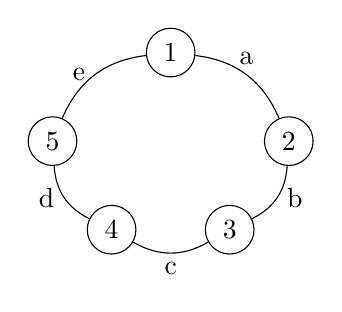
\begin{tikzpicture}[scale = 0.75]
          \node[draw, circle] at ( 0, 1.5)  (1) {1};
          \node[draw, circle] at ( 2, 0  )  (2) {2};
          \node[draw, circle] at ( 1,-1.5)  (3) {3};
          \node[draw, circle] at (-1,-1.5)  (4) {4};
          \node[draw, circle] at (-2, 0  )  (5) {5};

          \draw[-] (1) edge [bend left] node[anchor = south] {a} (2);
          \draw[-] (2) edge [bend left] node[anchor = west]  {b} (3);
          \draw[-] (3) edge [bend left] node[anchor = north] {c} (4);
          \draw[-] (4) edge [bend left] node[anchor = east]  {d} (5);
          \draw[-] (5) edge [bend left] node[anchor = east]  {e} (1);
        \end{tikzpicture}
      }
      % Cette ligne de commentaire semble être nécessaire pour que les figures soient affichées sur une ligne
      \subfigure[]
      {
        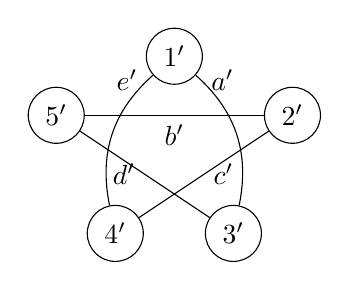
\begin{tikzpicture}[scale = 0.75]
          \node[draw, circle] at ( 0, 1.5)  (1) {$1'$};
          \node[draw, circle] at ( 2, 0.5)  (2) {$2'$};
          \node[draw, circle] at ( 1,-1.5)  (3) {$3'$};
          \node[draw, circle] at (-1,-1.5)  (4) {$4'$};
          \node[draw, circle] at (-2, 0.5)  (5) {$5'$};

          \draw[-] (1) edge [bend left] node[pos=0.05, anchor = west] {$a'$} (3);
          \draw[-] (2) edge node[anchor = north] {$b'$} (5);
          \draw[-] (2) edge node[pos=0.5, anchor = west] {$c'$} (4);
          \draw[-] (3) edge node[pos=0.5, anchor = east] {$d'$} (5);
          \draw[-] (1) edge [bend right] node[pos=0.05, anchor = east] {$e'$} (4);

        \end{tikzpicture}
      }
      % Cette ligne de commentaire semble être nécessaire pour que les figures soient affichées sur une ligne
      \subfigure[]
      {
        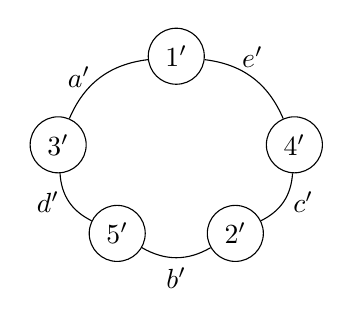
\begin{tikzpicture}[scale = 0.75]
          \node[draw, circle] at ( 0, 1.5)  (1) {$1'$};
          \node[draw, circle] at ( 2, 0  )  (4) {$4'$};
          \node[draw, circle] at ( 1,-1.5)  (2) {$2'$};
          \node[draw, circle] at (-1,-1.5)  (5) {$5'$};
          \node[draw, circle] at (-2, 0  )  (3) {$3'$};

          \draw[-] (1) edge [bend left] node[anchor = south] {$e'$} (4);
          \draw[-] (4) edge [bend left] node[anchor = west]  {$c'$} (2);
          \draw[-] (2) edge [bend left] node[anchor = north] {$b'$} (5);
          \draw[-] (5) edge [bend left] node[anchor = east]  {$d'$} (3);
          \draw[-] (3) edge [bend left] node[anchor = east]  {$a'$} (1);
        \end{tikzpicture}
      }
    \end{figure}
    Notons que les graphes \emph{b} et \emph{c} sont les mêmes, leurs noeuds ont simplement été réordonnés.\\
    L'isomorphisme entre \emph{a} et les deux autres est donné par : \\

    \begin{tabular}{lll}
      $f(1)=1'$ & $g(a)=e'$ \\
      $f(2)=4'$ & $g(b)=c'$ & $\varphi(a) = \{1, 2\}$\\
      $f(3)=2'$ & $g(c)=b'$ & $\varphi'(a') = \{1', 3'\}$\\
      $f(4)=5'$ & $g(d)=d'$ & $\varphi'(g(a)) = \{f(1), f(2)\}$\\
      $f(5)=3'$ & $g(e)=a'$ \\
    \end{tabular}
    \newline
    \newline
    \noindent
    Notons aussi que plusieurs résultats sont possibles : \\
    \begin{figure}[h!]
      \centering
      \subfigure[h!]
      {
        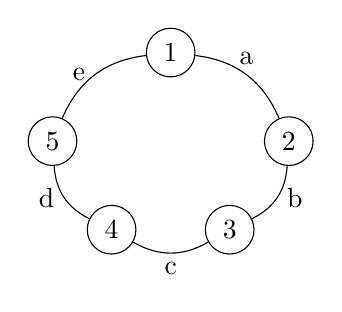
\begin{tikzpicture}[scale = 0.75]
          \node[draw, circle] at ( 0, 1.5)  (1) {1};
          \node[draw, circle] at ( 2, 0  )  (2) {2};
          \node[draw, circle] at ( 1,-1.5)  (3) {3};
          \node[draw, circle] at (-1,-1.5)  (4) {4};
          \node[draw, circle] at (-2, 0  )  (5) {5};

          \draw[-] (1) edge [bend left] node[anchor = south] {a} (2);
          \draw[-] (2) edge [bend left] node[anchor = west]  {b} (3);
          \draw[-] (3) edge [bend left] node[anchor = north] {c} (4);
          \draw[-] (4) edge [bend left] node[anchor = east]  {d} (5);
          \draw[-] (5) edge [bend left] node[anchor = east]  {e} (1);
        \end{tikzpicture}
      }
      % Cette ligne de commentaire semble être nécessaire pour que les figures soient affichées sur une ligne
      \subfigure[h!]
      {
        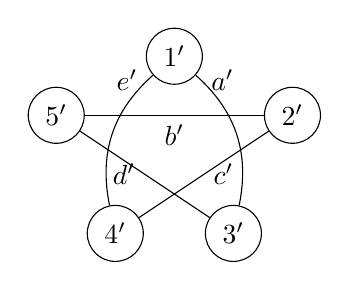
\begin{tikzpicture}[scale = 0.75]
          \node[draw, circle] at ( 0, 1.5)  (1) {$1'$};
          \node[draw, circle] at ( 2, 0.5)  (2) {$2'$};
          \node[draw, circle] at ( 1,-1.5)  (3) {$3'$};
          \node[draw, circle] at (-1,-1.5)  (4) {$4'$};
          \node[draw, circle] at (-2, 0.5)  (5) {$5'$};

          \draw[-] (1) edge [bend left] node[pos=0.05, anchor = west] {$a'$} (3);
          \draw[-] (2) edge node[anchor = north] {$b'$} (5);
          \draw[-] (2) edge node[pos=0.5, anchor = west] {$c'$} (4);
          \draw[-] (3) edge node[pos=0.5, anchor = east] {$d'$} (5);
          \draw[-] (1) edge [bend right] node[pos=0.05, anchor = east] {$e'$} (4);
        \end{tikzpicture}
      }
      \subfigure[h!]
      {
        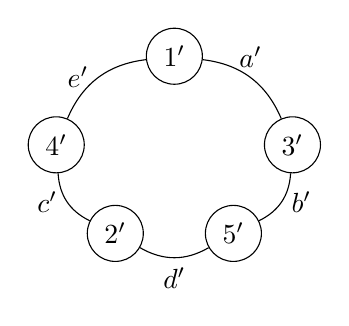
\begin{tikzpicture}[scale = 0.75]
          \node[draw, circle] at ( 0, 1.5)  (1) {$1'$};
          \node[draw, circle] at ( 2, 0  )  (3) {$3'$};
          \node[draw, circle] at ( 1,-1.5)  (5) {$5'$};
          \node[draw, circle] at (-1,-1.5)  (2) {$2'$};
          \node[draw, circle] at (-2, 0  )  (4) {$4'$};

          \draw[-] (1) edge [bend left] node[anchor = south] {$a'$} (3);
          \draw[-] (3) edge [bend left] node[anchor = west]  {$b'$} (5);
          \draw[-] (5) edge [bend left] node[anchor = north] {$d'$} (2);
          \draw[-] (2) edge [bend left] node[anchor = east]  {$c'$} (4);
          \draw[-] (4) edge [bend left] node[anchor = east]  {$e'$} (1);
        \end{tikzpicture}
      }
    \end{figure}

    \begin{tabular}{lll}
      $f(1)=1'$ & $g(a)=a'$ \\
      $f(2)=3'$ & $g(b)=b'$ \\
      $f(3)=5'$ & $g(c)=d'$ \\
      $f(4)=2'$ & $g(d)=c'$ \\
      $f(5)=4'$ & $g(e)=e'$ \\
    \end{tabular}
    \newline
    \newline
    Les six graphes de cet exemple sont isomorphes entre eux.\\
\end{myexem}

\subsection{Parcours eulérien}
\index{parcours}
\begin{mydef}
  Un \emph{parcours} est fermé si $v_0 = v_n$.
\end{mydef}

\index{chemin}
\begin{mydef}
  Un \emph{chemin} est un parcours dont tous les sommets sont distincts.
\end{mydef}

\index{cycle}
\begin{mydef}
  Un \emph{cycle} est un parcours fermé dont tous les sommets d'origine et intérieurs sont tous distincts.
\end{mydef}

\index{graphe!graphe connexe}
\begin{mydef}
  Un \emph{graphe} est \emph{connexe} si pour chaque pair de points il existe un parcours qui les relie. Les \emph{composantes connexes} d'un graphe sont ses sous-graphes connexes maximaux.
\end{mydef}

\index{parcours!parcours eulérien}
\index{graphe!graphe eulérien}
\begin{mydef}
  Un \emph{parcours} est \emph{eulérien} s'il visite chaque arête une et une seule fois. Un \emph{graphe} est \emph{eulérien} s'il existe un parcours eulérien fermé.
\end{mydef}

\begin{mytheo} [Théorème d'Euler]
  Un graphe connexe est eulérien ssi tous les sommets sont de degré pair.
  \begin{proof}
    \noindent
    \newline
    \fbox{$\Longrightarrow$}
    \newline
    Chaque arête incidente à un noeud $x$ est utilisé par le parcours eulérien:
    \begin{itemize}
      \item soit pour entrer dans $x$;
      \item soit pour en sortir.\\
    \end{itemize}
    A chaque arête entrante correspond une arête sortante (celle qui suit dans le parcours sauf pour la dernière et la première).\\
    Donc, il y a une bijection entre les arêtes entrantes et les arêtes sortantes.\\
    $\longrightarrow$ degré pair \\

    \noindent
    \fbox{$\Longleftarrow$}
    \newline
    On va construire un parcours eulérien :\\
    \begin{enumerate}
      \item On part d'un noeud arbitraire $x_0$.
      \item On prend une arête incidente à $x_0$, on arrive à un nouveau noeud.
      \item Par parité, il y a au moins une arête non utilisée, on la prend, etc... Quand il n'y a plus d'arête disponible, on est forcément arrivé à $x_0$.\\
    \end{enumerate}
    \begin{center}
      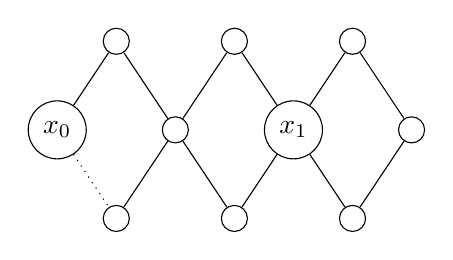
\begin{tikzpicture}[scale = 0.75]
        \node[draw, circle] at (-3, 0  )  (1)  {$x_0$};
        \node[draw, circle] at (-2, 1.5)  (2)  {};
        \node[draw, circle] at (-2,-1.5)  (3)  {};
        \node[draw, circle] at (-1, 0  )  (4)  {};
        \node[draw, circle] at ( 0, 1.5)  (5)  {};
        \node[draw, circle] at ( 0,-1.5)  (6)  {};
        \node[draw, circle] at ( 1, 0  )  (7)  {$x_1$};
        \node[draw, circle] at ( 2, 1.5)  (8)  {};
        \node[draw, circle] at ( 2,-1.5)  (9)  {};
        \node[draw, circle] at ( 3, 0  )  (10) {};

        \draw[-] (1) edge node {} (2);
        \draw[dotted] (1) edge node {} (3);
        \draw[-] (2) edge node {} (4);
        \draw[-] (3) edge node {} (4);
        \draw[-] (4) edge node {} (5);
        \draw[-] (4) edge node {} (6);
        \draw[-] (5) edge node {} (7);
        \draw[-] (6) edge node {} (7);
        \draw[-] (7) edge node {} (8);
        \draw[-] (7) edge node {} (9);
        \draw[-] (8) edge node {} (10);
        \draw[-] (9) edge node {} (10);
      \end{tikzpicture}
    \end{center}
    Pour tout autre noeud y, en arrivant à y, on a utilisé un nombre impair d'arêtes incidentes à y. On a un parcours fermé :
    \begin{itemize}
      \item Si toutes les arêtes incidentes aux x noeuds traversés par ce parcours sont utilisées, alors ce parcours est eulérien;
      \item Sinon, il y a $x_1 \in$ parcours avec au moins une arête non exploitée.\\
    \end{itemize}
    \begin{center}
      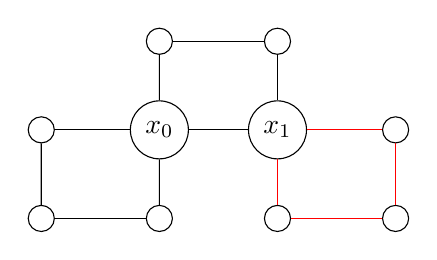
\begin{tikzpicture}[scale = 0.75]
        \node[draw, circle] at (-4, 0  )  (1)  {};
        \node[draw, circle] at (-4,-1.5)  (2)  {};
        \node[draw, circle] at (-2, 0  )  (3)  {$x_0$};
        \node[draw, circle] at (-2,-1.5)  (4)  {};
        \node[draw, circle] at (-2, 1.5)  (5)  {};
        \node[draw, circle] at ( 0, 1.5)  (6)  {};
        \node[draw, circle] at ( 0, 0  )  (7)  {$x_1$};
        \node[draw, circle] at ( 0,-1.5)  (8)  {};
        \node[draw, circle] at ( 2,-1.5)  (9)  {};
        \node[draw, circle] at ( 2, 0  )  (10) {};

        \draw[-] (1) edge node {} (2);
        \draw[-] (1) edge node {} (3);
        \draw[-] (2) edge node {} (4);
        \draw[-] (3) edge node {} (4);
        \draw[-] (3) edge node {} (5);
        \draw[-] (3) edge node {} (7);
        \draw[-] (5) edge node {} (6);
        \draw[-] (6) edge node {} (7);
        \draw[-, color=red] (7) edge node {} (8);
        \draw[-, color=red] (7) edge node {} (10);
        \draw[-, color=red] (8) edge node {} (9);
        \draw[-, color=red] (9) edge node {} (10);
      \end{tikzpicture}
    \end{center}
    On merge les deux parcours :\\
    $P_{0+1} = x_0 \rightarrow x_1 \textcolor{red}{\rightarrow} x_1 \rightarrow x_0$\\
    Et on fait ça en boucle jusqu'à avoir toutes les arêtes.
  \end{proof}
\end{mytheo}

\begin{mytheo} [Existence d’un parcours eulérien]
  Un graphe connexe possède un parcours eulérien ssi le nombre de noeuds de degré impair est zéro ou deux.
  \begin{proof}
    \noindent
    \newline
    \fbox{$\Longrightarrow$}
    \newline
    \begin{itemize}
      \item Si ce parcours eulérien est fermé, tous les degrés sont pairs;
      \item Si ce parcours eulérien est ouvert, tous les degrés sont pairs, sauf $deg(u)$ et $deg(v)$ qui sont impairs.\\
    \end{itemize}

    \noindent
    \fbox{$\Longleftarrow$}
    \newline
    \begin{itemize}
      \item Si tous les degrés sont pairs alors il existe un parcours eulérien fermé;
      \item Si deux degrés sont impairs et si on ajoute une arête $e$ entre $u$ et $v$ :\\
      $\rightarrow$ Tous les degrés sont pairs.\\
      $\rightarrow$ Il existe un parcours eulérien fermé.\\
      En retirant $e$, on obtient un parcours eulérien ouvert $u \rightarrow v$
    \end{itemize}
  \end{proof}
\end{mytheo}

\begin{mytheo} [Théorème des poignées de mains]
  La somme des degrés des noeuds d’un graphe est deux fois le nombre d’arêtes.\\
  $\sum_{v_i \in V}^{} deg(v_i) = 2|E|$
  \begin{proof}
    En utilisant la matrice d'incidence $M$ (voir \ref{in_matrix}), on peut calculer $\sum_{i,j}^{} M_{i,j}$ de deux façon différentes :\\
    \begin{tikzpicture}[decoration=brace]
      \matrix (m) [matrix of math nodes,left delimiter=[,right delimiter={]}] {
          0 & 1 & 1 & 0 & 1 & 0 \\
          1 & 1 & 0 & 1 & 0 & 1 \\
          1 & 0 & 0 & 1 & 0 & 1 \\
          0 & 0 & 1 & 0 & 1 & 0 \\
      };
      \draw[decorate,transform canvas={xshift=1.3em},thick] (m-1-6.north east) -- node[right=2pt] {$\sum_i \sum_j M_{ij} = \sum_{v_i \in V} deg(v_i)$} (m-4-6.south east);
      \draw[decorate,transform canvas={yshift=-1.7em},thick] (m-4-6.north east) -- node[below=2pt] {$\sum_i \sum_j M_{ij} = 2|E|$} (m-3-1.south west);
    \end{tikzpicture}
    \vspace*{5mm}
    \begin{center}
      $\sum_i \sum_j M_{ij} = \sum_i \sum_j M_{ij}$\\
      \vspace*{2mm}
      $2|E| = \sum_{v_i \in V} deg(v_i)$
    \end{center}
  \end{proof}
\end{mytheo}

\subsection{Représentation matricielle du graphe}
\index{matrice d'adjacence}
\begin{mydef}
  La \emph{matrice d'adjacence} est une matrice carrée $n$x$n$ dont l'élément $ij$ est le nombre d'arêtes entre les sommets $v_i$ et $v_j$.
\end{mydef}

\index{matrice d'incidence}
\begin{mydef}
  \label{in_matrix}
  La \emph{matrice d'incidence} est une matrice rectangulaire $n$x$m$ dont l'élément $ij$ est le nombre de fois que le sommet $v_i$ est incident à l'arête $e_j$.
\end{mydef}

\begin{myexem}
  \noindent
  \begin{center}
    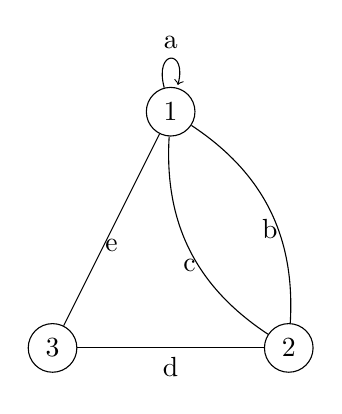
\begin{tikzpicture}[scale = 0.75]
      \node[draw, circle] at ( 0, 4)  (1)  {$1$};
      \node[draw, circle] at ( 2, 0)  (2)  {$2$};
      \node[draw, circle] at (-2, 0)  (3)  {$3$};

      \draw[-] (1) edge [loop above] node {a} (1);
      \draw[-] (1) edge [bend left] node [anchor = north] {b} (2);
      \draw[-] (1) edge [bend right] node [anchor = north] {c} (2);
      \draw[-] (2) edge node [anchor = north] {d} (3);
      \draw[-] (1) edge node [anchor = north] {e} (3);
    \end{tikzpicture}

    $
    Matrice\ d'adjacence\ :\ A\ = \bordermatrix{~ & 1 & 2 & 3 \cr
                                                1 & 1 & 2 & 1 \cr
                                                2 & 2 & 0 & 1 \cr
                                                3 & 1 & 1 & 0 \cr}
    $

    $
    Matrice\ d'incidence\ :\ M\ = \bordermatrix{~ & a & b & c & d & e\cr
                                                1 & 2 & 1 & 1 & 0 & 1\cr
                                                2 & 0 & 1 & 1 & 1 & 0\cr
                                                3 & 0 & 0 & 0 & 1 & 1\cr}
    $
  \end{center}
  $(A^k)_{ij} =$ nombre de parcours $i \to j$ de longueur $k$.\\
  $
    A^0\ =\ I\ =  \begin{pmatrix} 1 & 0 & 0\\
                                  0 & 1 & 0\\
                                  0 & 0 & 1
                  \end{pmatrix},\
    A^1\ =\ A\ =\begin{pmatrix} 1 & 2 & 1\\
                                2 & 0 & 1\\
                                1 & 1 & 0
                \end{pmatrix},\
    A^2\ = \begin{pmatrix}  6 & 3 & 3\\
                            3 & 5 & 2\\
                            3 & 2 & 2
            \end{pmatrix}
  $
\end{myexem}

\begin{mytheo} [Matrice d’adjacence et nombre de parcours]
  Soit $A$ la matrice d'adjacence d'un graphe. Alors l'élément $ij$ de $A^k$ ($k \geq 0$) est le nombre de parcours de longueur $k$ de $v_i$ vers $v_j$.
  \begin{proof}
    Nous procédons par récurrence. Soit $A$ une matrice d'adjacence.\\
    Pour $k=0$, $A^{0}=Id$. La propriété est vérifiée par convention. Il existe un chemin de longueur 0 d'un point vers lui même. \\
    Pour $k=1$, $A^{1}=A$ représente bien le nombre de parcours de longueur 1. \\
    Supposons la propriété vérifiée pour $A^{k}$.

    Nombre de parcours de parcours de $i \to j$ de longueur $k+1 =$\\
    $= \sum_{l \in E}$ (\# parcours de $i \to l$ de longueur $k$)$.$(\# arêtes $l \to j$)\\
    $= \sum_{l \in E} A_{il}^{k}.A_{lj}$\\
    $= A_{ij}^{k+1}$
  \end{proof}
\end{mytheo}

\index{distance entre deux noeuds}
\begin{mydef}
  La \emph{distance $d(u, v)$} entre les noeuds $u$ et $v$ d'un graphe est le nombre d'arêtes minimal d'un parcours entre ces deux noeuds.
\end{mydef}

\begin{mylem}
  Si $u...u'...v'...v$ est un parcours de longeur minimale de $u$ vers $v$, alors le sous-parcours $u'...v'$ est un parcours de longeur minimale de $u'$ vers $v'$.\\
  En particulier, un parcours de longueur minimale est toujours un chemin.
  \begin{proof}
    Si ce parcours entre $u'$ et $v'$ n'était pas le plus court, on utiliserait le parcours strictement plus court pour la construction du parcours entre $u$ et $v$.
  \end{proof}
\end{mylem}

\subsection{Graphe biparti}
\index{graphe!graphe biparti}
\begin{mydef}
  Un graphe est \emph{biparti}  s'il existe une partition en deux ensembles $V_1$ et $V_2$ tels que les sommets de $V_1$ ne sont adjacents qu'à des sommets de $V_2$ et vice versa. La bipartition est $(V_1, V_2)$.
\end{mydef}

\begin{myexem}
  \noindent
  \begin{center}
    \definecolor{myblue}{RGB}{80,80,160}
    \definecolor{mygreen}{RGB}{80,160,80}

    \begin{tikzpicture}[thick,
      every node/.style={draw,circle},
      fsnode/.style={fill=myblue},
      ssnode/.style={fill=mygreen},
      every fit/.style={ellipse,draw,inner sep=-2pt,text width=2cm},
      ->,shorten >= 3pt,shorten <= 3pt
    ]

    % the vertices of U
    \begin{scope}[start chain=going below,node distance=7mm]
    \foreach \i in {1,2,...,5}
      \node[fsnode,on chain] (f\i) [label=\i] {};
    \end{scope}

    % the vertices of V
    \begin{scope}[xshift=4cm,yshift=-0.5cm,start chain=going below,node distance=7mm]
    \foreach \i in {6,7,...,9}
      \node[ssnode,on chain] (s\i) [label=\i] {};
    \end{scope}

    % the set U
    \node [myblue,fit=(f1) (f5),label=$V_1$] {};
    % the set V
    \node [mygreen,fit=(s6) (s9),label=$V_2$] {};

    % the edges
    \draw (f1) -- (s6);
    \draw (s6) -- (f2);
    \draw (f2) -- (s7);
    \draw (s7) -- (f3);
    \draw (s8) -- (f3);
    \draw (f3) -- (s9);
    \draw (s9) -- (f5);
    \draw (f5) -- (s6);
    \draw (f4) -- (s9);
    \end{tikzpicture}
  \end{center}
\end{myexem}

\begin{mytheo} [Graphes bipartis]
  Un graphe est biparti ssi tous ses cycles sont de longueur paire.
  \begin{proof}
    \noindent
    \newline
    \fbox{$\Longrightarrow$}
    \newline
    Il existe une bipartition $(V_1,V_2)$.\\
    \begin{align*}
      Cycle : & V_1, V_2, V_3, ..., V_n \Rightarrow n\ est\ pair.\\
              & \downarrow\ \ \ \downarrow\ \ \ \downarrow\ \ \ \ \ \ \ \downarrow\\
              & V_1, V_2, V_1, ..., V_2
    \end{align*}

    \noindent
    \fbox{$\Longleftarrow$}
    \newline
    Partition d'un noeud $v_0$ au hasard.\\
    $V_0\ =\ \{v|d(v,\ v_0)\ $paire$\}$\\
    $V_1\ =\ \{v|d(v,\ v_0)\ $impaire$\}$\\
    C'est une partition. Est-ce une bipartition?
    Oui, sinon on aurait par exemple une arête $uv$ dans $V_0$.

    \begin{center}
      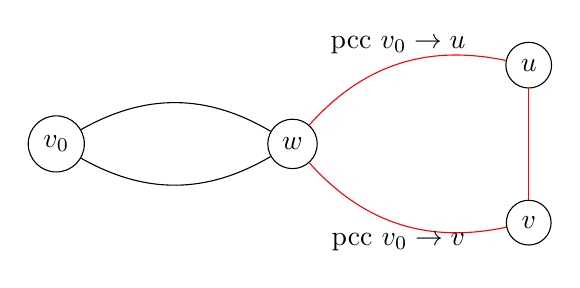
\begin{tikzpicture}
        \node[draw, circle] at (-4, 0)  (1)  {$v_0$};
        \node[draw, circle] at (-1, 0)  (2)  {$w$};
        \node[draw, circle] at ( 2, 1)  (3)  {$u$};
        \node[draw, circle] at ( 2,-1)  (4)  {$v$};

        \draw[-] (1) edge [bend left]  node {} (2);
        \draw[-] (1) edge [bend right] node {} (2);
        \draw[-, color=red] (2) edge [bend left]  node [anchor = south, color=black] {pcc $v_0 \to u$} (3);
        \draw[-, color=red] (2) edge [bend right] node [anchor = north, color=black] {pcc $v_0 \to v$} (4);
        \draw[-, color=red] (3) edge node {} (4);
      \end{tikzpicture}
    \end{center}
    pcc : plus court chemin.\\
    Les pcc sont de longueure paire car on est dans $V_0$.\\
    $w$ est le dernier point d'intersection entre les chemins $v_0 \to u$ et $v_0 \to v$.\\
    \textcolor{red}{$\triangle$} est un cycle de longueur impaire car $w \to u$ et $w \to v$ sont paires (les deux sous-chemins de $v_0 \to w$ sont des plus court chemin de même longueur) + une arête $uv$.\\
    $lg(wuvw)\ =\ lg(v_{0}uvv_0)\ - \ 2lg(v_0w)$\\
    $impaire\ \ \ \ \ \ \ \ \ \ \ \ \ \ \ \ \ \ \ \ \ \ \ \ \ \ \ \ \ \ paire$\\
    Contradiction, si arête dans $V_1$ même raisonnement.
  \end{proof}
\end{mytheo}
